\documentclass[11pt]{article}

\usepackage{amsmath}
\usepackage{amssymb}
\usepackage{amsthm}
\usepackage{hyperref}
\usepackage{microtype}
\usepackage{graphicx}
\graphicspath{ {./img/} }

\setlength{\parindent}{0cm}
\let\emptyset\varnothing

\title{\textbf{MATH 2135 Linear Algebra} \\ Chapter 1 Vector Spaces}
\author{Alyssa Motas}

\begin{document}

    \maketitle

    \pagebreak

    \tableofcontents

    \pagebreak

    \section{1.A Complex Numbers}

    \subsection{Complex numbers}

    \subsubsection{Definition}
    A complex number is a pair \((a,b)\) where \(a,b \in \mathbb{R}\). We write \(\mathbb{C}\) for the set of complex numbers. The set of all complex numbers is denoted by \(\mathbb{C}\): \[\mathbb{C} = \{a + bi \mid a,b \in \mathbb{R}\}.\]With the following operations:
    \begin{align*}
        (a,b) + (c,d)     &= (a+c, b+d)    \\
        (a,b) \cdot (c,d) &= (ac-bd,ad+bc) 
    \end{align*}

    We also define: \[0 = (0,0) \qquad 1 = (1,0).\]
    \emph{Claim.} The set \(\mathbb{C}\), together with \(0,1 \in \mathbb{C}\) and the operations \(+\) and \(\cdot\) defined above, is a field.

    \subsubsection{Notation}
    \begin{itemize}
        \item We write \(i = (0,1) \in \mathbb{C}.\)
        \item If $a$ is a real number, we will also write \(a = (a,0) \in \mathbb{C}\).
    \end{itemize}
    Note, if \(a,b\) are real numbers, then
    \begin{align*}
        a + bi &= (a,0) + (b,0) \cdot (0,1) \\
               &= (a,0) + (0,b)             \\
               &= (a,b).
    \end{align*}
    The notation \(a + bi\) is what everybody uses for complex numbers. With this notation, the rules of addition and multiplication become easier to understand and remember.
    \begin{align*}
        (a+bi)+(c+di) &= (a+c) + (b+d)i         \\
        (a+bi)(c+di)  &= ac + adi + bci + bdi^2 \\
                      &= ac + adi + bci - bd    \\
                      &= (ac - bd) + (ad + bc)i.
    \end{align*}
    Note: \(i^2 = i \cdot i = (0,1) \cdot (0,1) = (-1,0) = -1.\)

    \subsubsection{Terminology}
    Given a complex number \[z = a + bi = (a,b)\] the real number $a$ is called the \emph{real part} of $z$, and the real number $b$ is called the \emph{imaginary part} of $z$.

    \vspace{1em}

    The complex number \(\bar{z} = a - bi\) is called the \emph{complex conjugate} of $z$.
    \begin{align*}
        z \bar{z} &= (a+bi)(a - bi)                              \\
                  &= a^2 - abi + abi - b^2 i^2                   \\
                  &= a^2 + b^2 \qquad \text{which is \emph{real}}
    \end{align*}

    \subsubsection{Division Operation, Part I}
    It is easy to divide a complex number by a real number. \[\frac{a+bi}{c} = \frac{a}{c} + \frac{b}{c} i.\]

    \subsubsection{Division Operation, Part II}
    How do we divide a complex number by a complex number? For instance, \[\frac{a+bi}{z} \qquad \text{where } z = c + di.\] We can simply take the conjugate of $z$ and then we have \[\frac{a + bi}{z} = \frac{(a+bi)\bar{z}}{z \bar{z}} = \frac{(a+bi)(c-di)}{c^2 + d^2} \qquad \text{where } c^2 + d^2 \text{ is a real.}\]

    \subsubsection{Multiplicative Inverse}

    The multiplicative of a complex number \(z = a + bi\) is \[z^{-1} = \frac{1}{z} = \frac{\bar{z}}{z \bar{z}} = \frac{a - bi}{a^2 + b^2} = \frac{a}{a^2 + b^2} - \frac{b}{a^2 + b^2}i.\]

    \subsubsection{Argument of a complex number}\footnote{Taken from the \href{https://en.wikipedia.org/wiki/Argument_(complex_analysis)}{Wikipedia}.}
    The argument of $z$ is the angle between the positive real axis and the line joining the point to the origin. For each point on the plane, \(\arg\) is the function which returns the angle \(\phi\). The numeric value is given by the angle in radians, and is positive if measured counterclockwise.

    Algebraically, as any real quantity \(\phi\), such that \[z = r(cos \phi + i sin \phi) = r e^{i \phi}\] for some positive real $r$. The quantity $r$ is the modulus (or absolute value) of $z$, denoted $|z|$. \[r = \sqrt{x^2 + y^2}\]

    Some identities are \[\arg(zw) = \arg(z) + \arg(w) \mod{(-\pi, \pi]}\] \[\arg \left(\frac{z}{w}\right) = \arg(z) - \arg(w) \mod{(-\pi, \pi]}\] If \(z \neq 0\) and $n$ is any integer, then \[\arg(z^n) \equiv n \arg(z) \mod{(-\pi,\pi]}\]
    
    \emph{Example.} \[\arg \left(\frac{-1 -i}{i}\right) = \arg (-1 - i) - \arg (i) = - \frac{3 \pi}{4} - \frac{\pi}{2} = - \frac{5 \pi}{4}.\] \emph{Complex logarithm.} From \(z = |z| e^{i \arg(z)}\) or \(z = |z| e^{i \theta}\), it easily follows that \[\arg(z) = -i \ln \frac{z}{|z|}.\]

    \pagebreak

    \subsection{Fundamental Theorem of Algebra}

    Over the complex numbers, every non-constant polynomial has a root.
    \begin{itemize}
        \item There are two solutions (namely \(x = -2, 2\)) over \(\mathbb{R}\): \[x^2 - 4 = 0 \Leftrightarrow (x-2)(x+2) = 0 \]
        \item Has no roots over \(\mathbb{R}\): \[x^2 + 4 = 0.\]
        \item Has two solutions over \(\mathbb{C}\): \[z^2 + 4 = 0 \Leftrightarrow z^2 = -4 \Leftrightarrow z = \pm \sqrt{-4} = \pm 2i\] \[z^2 + 4 = (z - 2i)(z + 2i)\]
        \item Only one root over \(\mathbb{R}\): \[x^3 = 1\]
        \item Three distinct solutions over \(\mathbb{C}\): \[z^3 = 1\]
    \end{itemize}

    \subsection{Lists}

    \subsubsection{Definition}

    Suppose $n$ is a nonnegative integer. A \emph{list} of \emph{length} $n$ is an ordered collection of $n$ elements (which might be numbers, other lists, or more abstract entities) separated by commas and surrounded by parentheses. A list of length $n$ looks like this: \[(x_1, \dots, x_n).\] Two lists are equal if and only if they have the same length and the same elements in the same order.

    \subsubsection{Examples}
    \begin{itemize}
        \item The set \(\mathbb{R}^2\) is the set of all ordered pairs of real numbers: \[\mathbb{R}^2 = \{(x,y) \mid x,y \in \mathbb{R}\}.\]
        \item The set \(\mathbb{R}^3\) is the set of all ordered triples of real numbers: \[\mathbb{R}^3 = \{(x,y,z) \mid x,y,z \in \mathbb{R}\}.\]
        \item A list of length 0 looks like this: ().
        \item Lists differ from sets in two ways: in lists, order matters and repetitions have meaning; in sets, order and repetitions are irrelevant.
    \end{itemize}

    \subsection{\textbf{F}\(^n\)}

    \subsubsection{Definition}

    \(\textbf{F}^n\) is the set of all lists of length $n$ of elements of \textbf{F}: \[\textbf{F}^n = \{(x_1, \dots, x_n \mid x_j \in \textbf{F} \text{ for } j = 1, \dots, n)\}.\] For \((x_1, \dots, x_n) \in \textbf{F}^n\) and \(j \in \{1, \dots, n\}\), we say that \(x_j\) is the $j$th \emph{coordinate} of \((x_1, \dots, x_n).\)

    \subsubsection{Addition}
    Addition is defined by adding corresponding coordinates: \[(x_1, \dots, x_n) + (y_1, \dots, y_n) = (x_1 + y_1, \dots, x_n + y_n).\] It is also commutative.

    \subsubsection{0}
    Let 0 denote the list of length $n$ whose coordinates are all 0: \[0 = (0, \dots, 0).\]

    \subsubsection{Additive Inverse}
    For \(x \in \textbf{F}^n\), the \emph{additive inverse} of $x$, denoted $-x$, is the vector \(-x \in \textbf{F}^n\) such that \[x + (-x) = 0.\] In other words, if \(x = (x_1, \dots, x_n)\) then \(-x = (-x_1, \dots, -x_n).\)

    \subsubsection{Scalar Multiplication}
    The \emph{product} of a number \(\lambda\) and a vector in \(\textbf{F}^n\) is computed by multiplying each coordinate of the vector by \(\lambda\): \[\lambda (x_1, \dots, x_n) = (\lambda x_1, \dots, \lambda x_n);\] here \(\lambda \in \textbf{F}\) and \((x_1, \dots, x_n) \in \textbf{F}^n.\)

    \subsection{Digression on Fields}
    A \emph{field} is a set containing at least two distinct elements called 0 and 1, along with operations of addition and multiplication. Thus, \(\mathbb{R}\) and \(\mathbb{C}\) are fields, as is the set of rational numbers along with the usual operations. Another example of a field is the set \(\{0,1\}\) with the usual operations of addition and multiplication except that \(1+1\) is defined to equal 0.

    \pagebreak

    \section{1.B Definition of Vector Space}

    \subsection{Definition}

    Let \textbf{F} be a field. A \emph{vector space} over \textbf{F} is a set $V$, together with a distinguished element \(0 \in V\) and with operations 
    \begin{align*}
        \text{addition} \qquad              & + : V \times V \rightarrow V \\
        \text{scalar multiplication} \qquad & \cdot : \textbf{F} \times V \rightarrow V.
    \end{align*}
    Satisfies the following 8 axioms:
    \begin{enumerate}
        \item[(A1)] Commutativity of addition. \[\forall v,w \in V, v + w = w + v\] 
        \item[(A2)] Associativity of addition. \[\forall v,w,u \in V, (v+w)+u = v+(w+u)\]
        \item[(A3)] Additive identity. \[\forall v \in V, 0 + v = v\]
        \item[(A4)] Additive inverse. \[\forall v \in V, \exists w \in V, v + w = 0\]
        \item[(M1)] Multiplicative identity. \[\forall v \in V, 1v = v\]
        \item[(M2)] Left distributivity. \[\forall a \in F, \forall v,w \in V, a(v+w) = av + aw\]
        \item[(M3)] Right distributivity. \[\forall a,b \in F, \forall v \in V, (a+b)v = av + bv\]
        \item[(M4)] Associativity of multiplication. \[\forall a,b \in F, \forall v \in V, (ab)v = a(bv)\]    
    \end{enumerate}

    \subsubsection{Terminology}

    \begin{itemize}
        \item The elements of \textbf{F} are called \emph{scalars}.
        \item The elements of $V$ are called \emph{vectors or points}.
        \item A vector space over \(\mathbb{R}\) is called a \emph{real vector space}.
        \item A vector space over \(\mathbb{C}\) is called a \emph{complex vector space}.
    \end{itemize}

    \pagebreak

    \subsection{Examples of Vector Spaces}

    \begin{enumerate}
        \item[(1)] \(\textbf{F}^n\) is the set of column vectors (sometimes row vectors) with elements from \textbf{F}. For instance, \(\mathbb{R}^n\) and \(\mathbb{C}^n\) are such vector spaces.
        \begin{align*}
            \textbf{F}^n &= \left\{ \begin{bmatrix}
                                        a_1    \\
                                        a_2    \\
                                        \vdots \\
                                        a_n
                                    \end{bmatrix} \mid a_1, \dots, a_n \in \textbf{F} \right\} \\
                         &= \{(a_1, a_2, \dots, a_n) \mid a_1, \dots, a_n \in \textbf{F}\}     \\
            0            = \begin{bmatrix}
                                0      \\
                                0      \\
                                \vdots \\
                                0
                            \end{bmatrix} \qquad
            \begin{bmatrix}
                a_1    \\
                \vdots \\
                a_n
            \end{bmatrix} &+ \begin{bmatrix}
                                b_1    \\
                                \vdots \\
                                b_n
                            \end{bmatrix} = \begin{bmatrix}
                                                a_1 + b_1 \\
                                                \vdots    \\
                                                a_n + b_n 
                                            \end{bmatrix} \qquad
            k \begin{bmatrix}
                a_1    \\
                \vdots \\
                a_n
              \end{bmatrix} = \begin{bmatrix}
                  k a_1  \\
                  \vdots \\
                  k a_n
              \end{bmatrix}
        \end{align*}
        The properties of \(\textbf{F}^n\) makes it a vector space. 

        \item[(2)] Let \(\textbf{F}^{\infty} = \{(x_1,x_2,x_3,x_4, \dots) \mid x_1,x_2,\dots \in \textbf{F}\}\) be the set of inifnite sequences of scalars. We define the following:
        \begin{itemize}
            \item \(0 = (0,0,0,\dots)\) is the constant zero sequences.
            \item If \(x = (x_1, x_2, x_3, \dots)\) and \(y = (y_1,y_2,y_3, \dots)\) then we define \[x + y = (x_1 + y_1, x_2 + y_2, \dots).\]
            \item If \(k \in \textbf{F}\) and \(x = (x_1,x_2,x_3, \dots)\), then we define \[kx = (kx_1, kx_2, \dots).\]
        \end{itemize}
        Then \(\textbf{F}^{\infty}\) is a vector space.  

        \pagebreak

        \item[(3)] Let \textbf{F} be a field and let $S$ be a set. Define \(\textbf{F}^{S} = \{f : S \rightarrow \textbf{F} \mid \text{$f$ is a function from $S$ to \textbf{F}}\}.\)
        
        \vspace{1em}

        Define \(0 \in \textbf{F}^{S}\) by \(0(x) = 0\). The $f$ is the zero function, $x$ is any element in $S$, which gives the output of 0. 

        \vspace{1em}

        If \(f,g \in \textbf{F}^{S}\), define \(f + g \in \textbf{F}^{S} \) as \[(f+g)(x) = f(x) + g(x).\]
        \begin{center}
            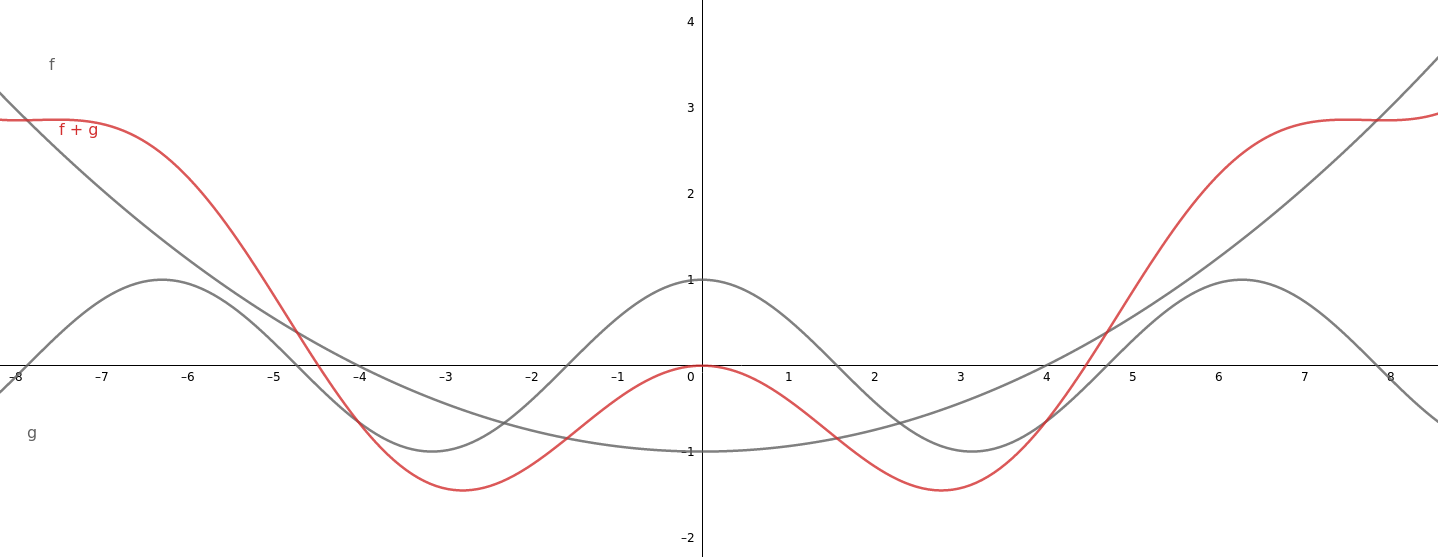
\includegraphics[width=\textwidth]{fg.png}
        \end{center}
        If \(k \in \textbf{F}\) and \(f \in \textbf{F}^{S}\), define \(kf \in \textbf{F}^{S}\) as \[(kf)(x) = k(f(x)).\]
        \begin{center}
            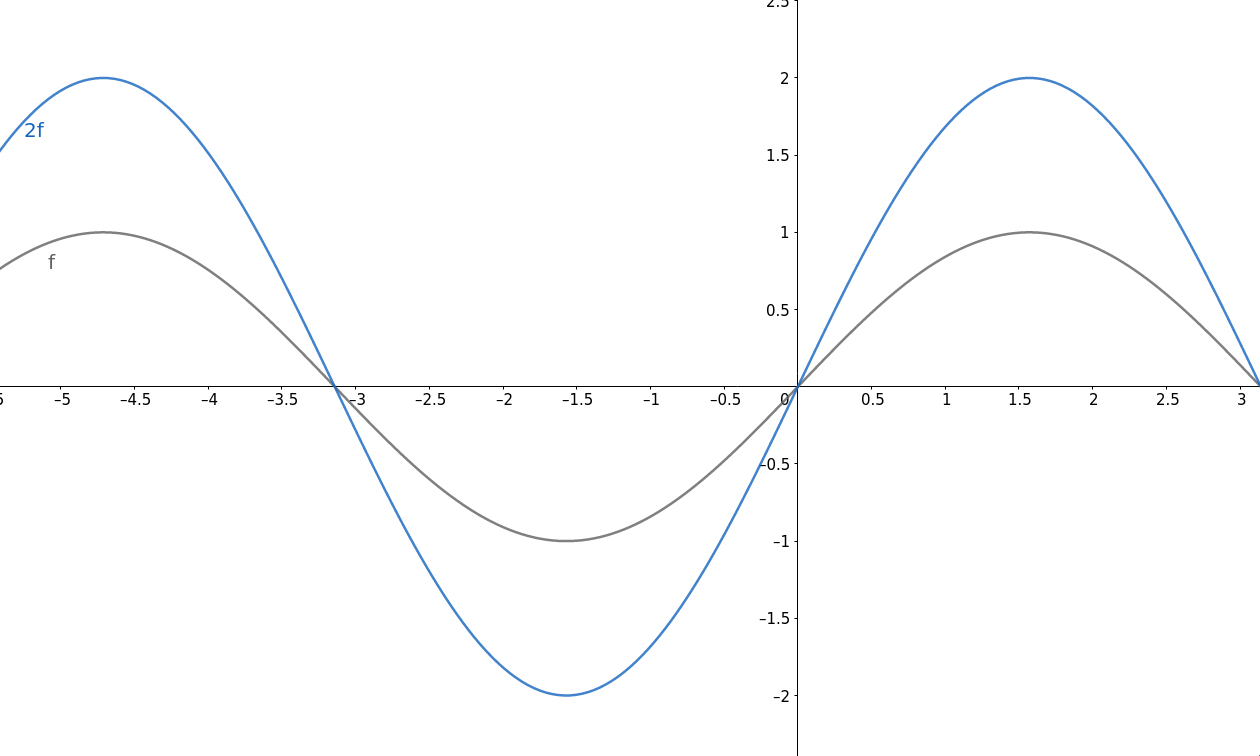
\includegraphics[width=10cm]{2f.png}
        \end{center}
        Then \(\textbf{F}^{S}\) is a vector space.

        \vspace{1em}

        \emph{Note:} The functions \(F,G : X \rightarrow Y\) are equal if \[\forall x \in X, F(x) = G(x).\]

        \begin{proof}
            Take arbitrary \(f,g \in \textbf{F}^{S}\). We have to show that \(f + g = g + f\) or \(\forall x \in S, (f + g)(x) = (g + f)(x).\) Suppose we take an arbitrary \(x \in S\), then we have
            \begin{align*}
                (f+g)(x) &= f(x) + g(x)                                       \\
                         &= g(x) + f(x) \quad \text{ by properties of fields} \\
                         &= (g+f)(x).
            \end{align*}  
            This finishes the proof of (A1). The other field axioms are similar.
        \end{proof}

        \item[(4)] For a field \textbf{F}, we define \(\mathcal{P}(\textbf{F})\) as the set of all formal polynomials with variable \(x\) and coefficients in \textbf{F}. \[\mathcal{P}(\textbf{F}) = \{a_0 + a_1 x + a_2 x^2 + \dots + a_n x^n \mid n \leq 0, a_0, \dots, a_n \in \textbf{F}\}.\] An example would be \(\mathcal{P}(x) = 3 + 5x - 7x^2.\)
        
        \vspace{1em}

        There are two ways to think about a polynomial: ``formal'' or ``function.'' For example, define the two following polynomials over \(\mathbb{Z}_2\) \[p(x) = x + 1 \qquad q(x) = x^2 + 1.\] As a function, it would be equal since:
        \begin{center}
            \begin{tabular}{| c | c | c |} \hline
                $x$ & $p(x)$ & $q(x)$ \\ \hline
                0   &   1    &   1    \\ \hline
                1   &   0    &   0    \\ \hline    
            \end{tabular}
        \end{center}
        As a formal polynomial, it would be different because it has the following form:
        \begin{align*}
            p(x) &= 0x^2 + 1x + 1 \\
            q(x) &= 1x^2 + 0x + 1.
        \end{align*}

        \pagebreak

        To prove that \(\mathcal{P}(\textbf{F})\) is a vector space, let us define the following:
        \begin{itemize}
            \item Zero polynomial. \[\mathcal{P}(x) = 0\]
            \item Addition.
            \begin{align*}
                p(x)        &= a_0 + a_1x + a_2 x^2 + \dots + a_n x^n \\
                q(x)        &= b_0 + b_1x + b_2 x^2 + \dots + b_n x^n \\
                \cline{1-2}
                (p + q)(x)  &= (a_0 + b_0) + (a_1 + b_1)x + (a_2 + b_2)x^2 + \dots + (a_n + b_n) x^n
            \end{align*}
            \item Scalar multiplication. \[kp(x) = (ka_0) + (ka_1)x + (ka_2) x^2 + \dots + (k a_n) x^n\]
        \end{itemize}
        With these operations, \(\mathcal{P}(\textbf{F})\) is a vector space.
    \end{enumerate}

    \subsection{Properties of Vector Spaces}

    Let $V$ be a vector space over a field \textbf{F}.
    \begin{itemize}
        \item The additive identity is unique. In other words, if \(u \in V\) is an additive identity (satisfying \(\forall v \in V, u + v = v\)) then \(u = 0\).
        \item Additive inverses are unique. Therefore, we can write \(-v\) for the additive inverse of \(v\). We also use related notations such as \(v-w\) to mean \(v + (-w)\).
        \item Cancellation of addition. \[v + w = u + w \Rightarrow v = u\]
        \item For all \(v \in V\), we have \[0v = 0.\] The 0 is a scalar being multiplied by $v$ (vector), and the 0 on the right is the zero vector.
        \begin{proof}
            We have
            \begin{align*}
                0v + 0v &= (0 + 0)v && \text{by (M3)}                  \\
                        &= 0v       && \text{by properties of scalars} \\
                        &= 0 + 0v   && \text{by (A3)}
            \end{align*}
            So \(0v = 0\) follows by cancellation.
        \end{proof}
        \item For all scalars \(a \in \textbf{F}\), we have \[a0 = 0.\]
        \begin{proof}
            We have
            \begin{align*}
                a0 + a0 &= a(0 + 0) && \text{by (M2)} \\
                        &= a0       && \text{by (A3)} \\
                        &= 0 + a0   && \text{by (A3)}
            \end{align*}
            So \(a0 = 0\) follows by cancellation.
        \end{proof}
        \item For all \(v \in V\), we have \[(-1)v = -v.\]
        \begin{proof}
            We have
            \begin{align*}
                (-v) + v &= v + (-v) && \text{by (A1)} \\
                         &= 0.       && \text{by (A4)}
            \end{align*}
            We also have
            \begin{align*}
                (-1)v + v &= (-1)v + 1v && \text{by (M1)} \\
                          &= (-1 + 1)v  && \text{by (M3)} \\
                          &= 0v         && \text{by properties of scalars} \\
                          &= 0.         && \text{by a previously proved property}
            \end{align*}
            In particular, \[(-v) + v = (-1)v + v.\] Then the claim \(-v = (-1)v\) follows by cancellation.
        \end{proof}
    \end{itemize}

    \pagebreak

    \section{1.C Subspaces}

    \subsection{Definition}

    Let $V$ be a vector space over a field $F$. A subset $U$ of $B$ is called a \emph{subspace} of $V$ if $U$ is also a vector space in its own right, using the same zero, addition, and scalar multiplication as $V$.

    \subsubsection{Characterization of Subspaces}

    A subset $U \subseteq V$ is a subspace if and only if $U$ satisfies the following three conditions:

    \begin{enumerate}
        \item[(1)] Additive identity. \[0 \in U\]
        \item[(2)] Closed under addition. \[\forall v,w, v,w \in U \Rightarrow v + w \in U\] 
        \item[(3)] Closed under scalar multiplication. \[\forall a,v, a \in F, v \ in U \Rightarrow av \in U\] 
    \end{enumerate}
    \begin{proof}
        ``\(\Rightarrow\)'' Given \(U \subseteq V\), assume $U$ is a subspace of $V$. We want to show that $U$ satisfies all three conditions above.
        \begin{enumerate}
            \item[(1)] By definition of subspaces, the zero vector of $V$ is the zero vector of $U$. So \(0 \in U\).
            \item[(2)] Since $U$ is a vector space, the sume of two vectors in $U$ is a vector in $U$. Also, $U$ uses the same addition operation as $V$. So whenever \(v,w \in U\), then \(v + w \in U.\)
            \item[(3)] Similar to (2).  
        \end{enumerate}
    \end{proof}

    \begin{proof}
        ``\(\Leftarrow\)'' Another proof is this: To show that $U$ is a vector space, we first need an element \(0 \in U\) and operations \[+ : U \times U \rightarrow U \qquad \text{and} \qquad \cdot : F \times U \rightarrow U.\] Second, we must show axioms (A1) - (M4).
        \begin{enumerate}
            \item[(1)] By assumption, \(0 \in U\), where 0 is the additive identity of $V$. So we can use 0 as the additive identity of $U$.
            \item[(2)] By assumption, $U$ is closed under addition, so the addition function \(+ : V \times V \rightarrow V\) restricts to a function \(+ : U \times U \rightarrow U.\) We can use the same function as the addition function on $U$. 
            \item[(3)] We do the same with scalar multiplication. 
        \end{enumerate}
        Second: We must show (A1) - (M4) hold. We only do (A1) since the rest are similar. To prove (A1), take arbitrary \(u,v \in U\). We need to show that \[u + v = v + u\] in $U$. But since $V$ is a vector space, we know that \[u + v = v + u\] in $V$. This automatically holds.

        \vspace{1em}

        The other parts of the definition of a vecotr space, such as associativity and commutativity, are automatically satisfied for $U$ because they hold on the larger space $V$. Thus, $U$ is a vector space and hence is a subspace of $V$.
    \end{proof}

    \subsection{Examples of Subspaces}

    \begin{enumerate}
        \item[(a)] Let \(V = \mathbb{R}^4\) and let \[W = \{ (x,y,z,w) \mid x = 3y + 2z \}.\] Then $W$ is a subspace of $V$.
        \begin{proof}
            We need to show that $W$ is a subspace of $V$.
            \begin{enumerate}
                \item[(1)] \((0,0,0,0) \in W\).
                \item[(2)] Assume \(v = (x,y,z,w) \in W\) and \(v' = (x',y',z',w') \in W.\) We need to show that \[x + x' = 3(y + y') + 2(z + z').\] We know that \(v \in W\) implies \[x = 3y + 2z.\] And we know that \(v' \in W\) implies \[x' = 3y' + 2z'.\] Add these two equations together and we get \[x + x' = 3(y + y') + 2(z + z').\]
                \item[(3)] Similar proof for scalar multiplication. 
            \end{enumerate}
        \end{proof} 

        \item[(b)] Recall that \(V = \mathbb{R}^{[0,1]}\) is the vector space of functions from the unit interval \[[0,1] = \{x \in \mathbb{R} \mid 0 \leq x \leq 1\}\] to \(\mathbb{R}.\) Let \(W = \{f : [0,1] \rightarrow \mathbb{R} \mid \text{ $f$ is continuous }\}.\) Then $W$ is a subspace of $V$.
        \begin{proof}
            We need to show that $W$ is a subspace of $V$.
            \begin{enumerate}
                \item[(1)] The zero function \(f(x) = 0\) is continuous. From Calculus, any constant function is continuous.
                \item[(2)] The sum of two continuous functions is continuous. This is from Calculus.
                \item[(3)] If $f$ is continuous, then so is $kf$, for any $k \in \mathbb{R}.$ This is also from Calculus.   
            \end{enumerate}
        \end{proof} 

        \item[(c)] Again, let \(V = \mathbb{R}^{[0,1]}\), and \(U = \{f: [0,1] \rightarrow \mathbb{R} \mid \text{ $f$ is differentiable }\}.\) Then $U$ is a subspace of $V$.
        \begin{proof}
            From Calculus, we know these hold true:
            \begin{enumerate}
                \item[(1)] The zero function \(f(x) = 0\) is differentiable with the derivative of \[f'(x) = 0.\]
                \item[(2)] If $f,g$ are differentiable then so is $f+g$ and \[(f+g)' = f' + g'.\]
                \item[(3)] If $f$ is differentiable and $k$ is a scalar, then $kf$ is differentiable. \[(kf)' = kf'.\]  
            \end{enumerate}
            For example, the derivative of \((0 + 2 \sin(x) - 3 \cos(x))' = 0 + 2 \cos(x) - 3(-\sin(x))\).

            We also know from Calculus that every differentiable function is continuous.
            \[U \subseteq W \subseteq V\] where $U$ is the set of all differentiable functions, $W$ is the set of all continuous functions, and $V$ is the set of all functions.
        \end{proof} 

        \item[(d)] Let \(V = \mathbb{R}^{[0,1]}\) and define \[X = \left\{ f:[0,1] \rightarrow \mathbb{R} \mid \text{ $f$ is differentiable and $f' \left( \frac{1}{2} \right) = 0$}\right\}.\] We claim that $X$ is a subspace of $V$.
        
        \emph{Note.} We already know that $U$, the set of differentiable functions, is a subspace of $V$.
        
        \begin{proof}
            Effectively, it is sufficient to show that $X$ is a subspace of $U$.
            \begin{enumerate}
                \item[(1)] The zero function \(f(x) = 0\) is differentiable since \[f'(x) = 0 \text{ and } f'\left(\frac{1}{2}\right) = 0.\] So \(f \in X\).
                \item[(2)] Given \(f,g \in X\), we must check that \(f + g \in X\). Clearly \(f + g\) is differentiable. We must check that \((f + g)' \left( \frac{1}{2} \right) = 0.\) From Calculus, we have
                \begin{align*}
                    (f+g)'\left(\frac{1}{2}\right) &= f'\left(\frac{1}{2}\right) + g' \left(\frac{1}{2}\right) \\
                    &= 0 + 0 \\
                    &= 0.
                \end{align*}
                So we have \(f + g \in X\).
                \item[(3)] Similar proof as follows for scalar multiplication: \[ (kg)' \left(\frac{1}{2}\right) = k \cdot f' \left(\frac{1}{2}\right) = 0. \] 
            \end{enumerate}
        \end{proof}

        \item[(e)] Let \(V = \mathbb{R}^{\infty}\), the set of infinite sequences of real numbers. \[\mathbb{R}^{\infty} = \{(a_0,a_1,a_2,a_3, \dots) \mid a_0,a_1, \dots \in \mathbb{R}\}.\] Recall that $V$ is a vector space. Let $W \subseteq V$ be the set of \emph{convergent} sequences. From Calculus, we know that some sequences converge and some do not.
        
        Some examples are:
        \begin{itemize}
            \item \(a_i = i \Rightarrow (0,1,2,3,4,5,6,7, \dots)\) \[\lim_{i \to \infty} a_i =\text{ does not exist, so it does not converge}\]
            \item \(b_i = \frac{1}{i} \Rightarrow (\frac{1}{1}, \frac{1}{2}, \frac{1}{3}, \dots)\) \[ \lim_{i \to \infty} b_i = \text{ converges to 0} \]
            \item \(c_i = (-1)^i \Rightarrow (1, -1, 1, -1, 1, -1, \dots)\) does not converge.
            \item \(d_i = 2 + \left( - \frac{1}{2} \right)^i \Rightarrow (3, 1.5, 2.25, 1.875, \dots)\) \[\lim_{i \to \infty} d_i = \text{ converges to 2}\]
        \end{itemize}
        Then $W$ is a subspace of $V$.

        \begin{proof}
            We must show that this is true.
            \begin{enumerate}
                \item[(1)] The zero sequence \(a_i = 0 \Rightarrow (0,0,0,\dots)\) converges to 0.
                \item[(2)] From Calculus, the sum of two convergent sequences converges. In fact, \[\lim_{i \to \infty} (a_i + b_i) = \lim_{i \to \infty} a_i + \lim_{i \to \infty} b_i\]
                \item[(3)] Similar proof to scalar muiltiplication. \[\lim_{i \to \infty} (ka_i) = k \lim_{i \to \infty} a_i\]   
            \end{enumerate}
        \end{proof}
        Let $U$ be the set of sequences that converge to 0. Then $U$ is a subspace of $V$ (and of $W$).

        \item[(f)] A reccurence relation. Consider the Fibonacci sequence \[1,1,2,3,5,8,13,21,34,55,89,144,\dots\] Let \(F_n\) be the \(n\)th element of this sequence. Then, we have the following recurrence:
        \begin{align*}
            \text{base case }  F_0 &= 1 \\
            \text{base case }  F_1 &= 1 \\
            \text{reccurence }  F_{n + 2} &= F_n + F_{n + 1} \qquad \text{for all } n \geq 0.
        \end{align*} 
        If we forget the base cases, we can consider the set of \emph{all} sequences satisfying the reccurence \[U = \{(a_0, a_1, a_2, \dots) \mid \text{ for all } n \geq 0, a_{n + 2} = a_n + a_{n+1}\}\] A sequence of numbers is called a \emph{generalized Fibonacci sequence} if it satisfies this reccurence, i.e. if it is a member of the set $U$.

        \emph{Examples.}
        \begin{align*}
            & 1,2,3,5,8,13, \dots \\
            & 7, -3,4,1,5,6,11,17,28,45, \dots \\
            & 0,0,0,0,0,0,0,0, \dots
        \end{align*} 

        \emph{Claim.} $U$ is a subspace of \(\mathbb{R}^{\infty}\).
        \begin{enumerate}
            \item[(1)] The sequence \(0,0,0, \dots\) is a generealized Fibonacci sequence.
            \item[(2)] $U$ is closed under addition.
            \begin{align*}
                & 1,2,3,5,8,13 \dots \\
                & 7, -3,4,1,5,6, \dots \\
                \cline{1-2}
                & 8,-1,7,6,13,19, \dots
            \end{align*}
            \begin{proof}
                Suppose \(a = (a_0, a_1, a_2, \dots) \in U\) and \(b = (b_0, b_1, b_2, \dots) \in U.\) Then \(a + b = c = (c_0, c_1, c_2, \dots)\) where \(c_i = a_i + b_i.\) 

                We must show \(c \in U\), i.e. we must show that $c$ is a generalized Fibonacci sequence.

                So take an arbitrary \(n \geq 0\). We must show \(C_{n+2} = C_n + C_{n+1}\). Indeed, we have:
                \begin{align*}
                    C_{n+2} &= a_{n+2} + b_{n+2} \\
                            &= (a_n + a_{n+1}) + (b_n + b_{n+1}) \\
                            &= (a_n + b_n) + (a_{n+1} + b_{n+1}) \\
                            &= c_n + c_{n+1}
                \end{align*}
            \end{proof}
            \item[(3)] Closed under scalar multiplication: similar.
        \end{enumerate}
    \end{enumerate}

    \subsection{Intersection of Subspaces}

    \subsubsection{Theorem}

    Let $V$ be a vector space over a field $F$. Assume $U$ and $W$ are subspaces of $V$. Then \(U \cap W\) is a subspace of $V$.

    \begin{proof}
        To show that \(U \cap W\) is a subspace, we need to show the three properties.
        \begin{enumerate}
            \item[(1)] We must show that \(0 \in U \cap W\). But by assumption, $U$ is a subspace, so \(0 \in U\). Also, $W$ is a subspace, so \(0 \in W\). By definiton of intersection, we have \(0 \in U \cap W\).
            \item[(2)] We must show that \(U \cap W\) is closed under addition. Consider arbitrary \(v,w \in U \cap W\) and we need to show that \(v + w \in U \cap W\).
            
            Indeed, we have:
            \begin{itemize}
                \item Since \(v \in U \cap W\), we know \(v \in U\).
                \item Since \(w \in U \cap W\), we know \(w \in U\).
                \item Since $U$ is a subspace, it is closed under addition, so \(v + w \in U\).
            \end{itemize}

            Similarly:
            \begin{itemize}
                \item Since \(v \in U \cap W\), we know \(v \in W\).
                \item Since \(w \in U \cap W\), we know \(w \in W\).
                \item Since $W$ is a subspace, it is closed under addition, so \(v + w \in W\).
            \end{itemize}

            From \(v + w \in U\) and \(v + w \in W\), by definition of intersection, we know \[v + w \in U \cap W.\]

            \item[(3)] We must show that \(U \cap W\) is closed under scalar multiplication. So consider arbitrary \(k \in F\) and \(v \in U \cap W\). We must show that \(kv \in U \cap W.\)
            
            Since \(v \in U \cap W\), we have \(v \in U\). Since $U$ is a subspace of $V$, we know that $U$ is closed under scalar multiplication, so $kv \in U$.

            Similarly, since \(v \in U \cap W\), we know \(v \in W.\) Since $W$ is a subspace of $V$, we know that $W$ is closed under scalar multiplication, so $kv \in W$.

            From \(kv \in U\) and \(kv \in W\), it follows that \(kv \in U \cap W\) (by definition of intersection), as desired.
        \end{enumerate}
    \end{proof}

    \subsubsection{Notations}

    \begin{itemize}
        \item \((x_1, \dots, x_n)\) is called an $n$-tuple.
        \item \((x_i)_{i \in \{1, \dots, n\}}\) is another notation for the same thing. This is called ``family'' notation. But, this notation also works for infinite index sets. \[ (x_i)_{i \in \mathbb{N}} = (x_0, x_1, x_2, \dots) \] \[ \left( \frac{1}{i + 1} \right)_{i \in \mathbb{N}} = \left( 1, \frac{1}{2}, \frac{1}{3}, \frac{1}{4}, \dots \right) \]
        \item More generally, we can use the ``family notation'' for other families of things, not necessarily numbers. 
        \begin{align*}
            U_1, U_2, U_3 && \text{3 subspaces of $V$} \\
            (U_i)_{i \in \{ 1,2,3 \}} && \text{Notation for the same thing.} \\
            (U_i)_{i \in I} && \text{Some family of subspaces.}
        \end{align*}

        \pagebreak
        
        \item Other notations that go along with these:
        \begin{itemize}
            \item Summation. \[\sum_{i \in \mathbb{N}} x_i\]
            \item Product. \[\prod_{i \in \mathbb{N}} x_i \]
            \item Limit. \[\lim_{i \to \infty} x_i\]
            \item Union. \[ \bigcup_{i \in \{1,2,3\}} U_i \]
            \item Intersection. \[ \bigcap_{i \in I} U_i\] 
        \end{itemize}
    \end{itemize}

    \subsubsection{Theorem}

    Let $V$ be a vector space over a field $F$. Let $I$ be a set. Let \((U_i)_{i \in I}\) be a \emph{family} of subspaces of $V$. Then, \[\bigcap_{i \in I} U_i\] is a subspace of $V$.

    \begin{proof}
        Let \(W = \bigcap_{i \in I} U_i\). To show that $W$ is a subspace of $V$, we must show the three subspace properties.
        \begin{enumerate}
            \item[(1)] We must show that \(0 \in W\). Take an arbitrary \(i \in I\). By assumption, \(U_i\) is a subspace of $V$. Therefore, \(0 \in U_i\).
            
            Since $i$ was arbitrary, we have \(0 \in U_i\) for all $i$, and therefore, by definition of intersection, \(0 \in \bigcap_{i \in I} U_i = W\).

            \item[(2)] Must show $W$ is closed under addition. Take an arbitrary \(v,u \in W\). We must show that \(v + u \in W\) or \(v + u \in \bigcap_{i \in I} U_i\).
            
            Take an arbitrary \(i \in I\). We must show that \(v + u \in U_i\). By assumption, \(v \in W = \bigcap_{i \in I} U_i\), therefore \(v \in U_i\).

            Simiarly, by assumption, \(u \in W = \bigcap_{i \in I} U_i\), therefore \(u \in U_i\).

            Also by assumption, \(U_i\) is a subspace of $V$, therefore it is closed under addition. So \(v + u \in U_i\).

            Since $i$ was arbitrary, we therefore know for all \(i \in I\) that \(v + u \in U_i\). It follows that \(v + u \in \bigcap_{i \in I} U_i\) as desired.

            \item[(3)] Closed under scalar multiplication: similar proof.
        \end{enumerate}
    \end{proof}

    \subsubsection{Meta-theorem}

    Let $V$ be a vector space over a field $F$. Let $P$ be any property of subspaces of $V$ such that $P$ is closed under arbitrary intersections.

    This means that whenever we have a family of subspaces, \((U_i)_{i \in I}\) of $V$,
    \begin{itemize}
        \item If, for all \(i \in I\), \(U_i\) has the property $P$, then \[\bigcap_{i \in I} U_i\] has the property $P$.
    \end{itemize}
    Then there exists a \emph{smallest} subspace of $V$ with the property $P$.

    \begin{proof}
        Let $P$ be such a property, i.e. a property of subspaces of $V$ that is closed under intersections.

        We want to showt hat there exists a \emph{smallest} subspace $W$ of $V$ with property $P$. Specifically, this means:
        \begin{enumerate}
            \item[(1)] $W$ is a subspace of $V$ and has the property $P$.
            \item[(2)] Whenever $W'$ is a subspace of $V$ that has the property $P$, then $W \subseteq W'$.  
        \end{enumerate}

        To show it, let \((U_i)_{i \in I}\) be the family of \emph{all} subspaces of $V$ satisfying property $P$. Define \[W = \bigcap_{i \in I} U_i. \] We have to show (1) and (2).

        \begin{enumerate}
            \item[(1)] $W$ is a subspace of $V$ by the previous theorem. Also, $W$ has the property $P$ because all $U_i$ have the property $P$ and $P$ is closed under intersections.
            \item[(2)] We must show that $W$ is smallest. So consider any subspace $W'$ with property $P$. We must show that \(W \subseteq W'\).
            
            But the family \((U_i)_{i \in I}\) contains \emph{all} subspaces with property $P$. So \(W' = U_i\) for all some \(i \in I\). Then \[W = \bigcap_{i \in I} U_i \subseteq U_i = W'.\]
        \end{enumerate}
    \end{proof}

    \subsubsection{Example}
    
    Consider \(v_1, v_2, v_3 \in V\).

    There exists a \emph{smallest subspace} $W$ of $V$ such that \(v_1, v_2, v_3 \in W\). We normally call $W$ the \emph{span} of \(v_1, v_2, v_3\).

    \begin{proof}
        By the meta-theorem, the property ``contains \(v_1, v_2\), and \(v_3\)'' is closed under intersections.
    \end{proof}
    
    \subsection{Sums of Subspaces}

    \subsubsection{Definition of Sum of Subsets}

    Suppose \(U_1, \dots, U_m\) are subsets of $V$. The \textbf{sum} of \(U_1, \dots, U_m\), denoted \(U_1 + \dots + U_m\), is the set of all possible sums of elements of \(U_1, \dots, U_m\). More precisely, \[U_1 + \dots + U_m = \{u_1 + \dots + u_m \mid u_1 \in U_1, \dots, u_m \in U_m\}.\]

    \subsubsection{Example}

    For \(U = \{(x,0,0) \in \textbf{F}^3 \mid x \in \textbf{F}\}\) and \(W = \{(0,y,0) \in \textbf{F}^3 \mid y \in \textbf{F}\}\), we have \[U + W = \{(x,y,0) \mid x,y \in \textbf{F}\}.\]

    For \(U = \{(x,x,y,y) \in \textbf{F}^4 \mid x,y \in \textbf{F}\}\) and \(W = \{(x,x,x,y) \in \textbf{F}^4 \mid x,y \in \textbf{F}\}\), then \[U + W = \{(x,x,y,z) \in \textbf{F}^4 \mid x,y,z \in \textbf{F}\}.\]

    \subsubsection{Sum of subspaces is the smallest containing subspace}

    Suppose \(U_1, \dots, U_m\) are subspaces of $V$. Then \(U_1 + \dots + U_m\) is the smallest subspace of $V$ containing \(U_1, \dots, U_m\).

    \begin{proof}
        We know that \(0 \in U_1 + \dots + U_m\) and \( U_1 + \dots + U_m \) is closed under addition and scalar multiplication. Thus, \(U_1 + \dots + U_m\) is a subspace of $V$.

        \(U_1, \dots, U_m\) are contained in \(U_1 + \dots + U_m\), and every subspace of $V$ containing \(U_1, \dots, U_m\) contains \(U_1 + \dots + U_m\).

        Thus, \(U_1 + \dots + U_m\) is the smallest subspace of $V$ containing \(U_1, \dots, U_m\).
    \end{proof}

    \emph{Note.} Sums of subspaces in theory of vector spaces are analogous to unions of subsets in set theory. Given two subspaces of a vector space, the smallest subspace containing them is their sum. Analogously, given two subsets of a set, the smallest subset containing them is their union.

    \subsection{Direct Sums}

    Suppose \(U_1, \dots, U_m\) are subspaces of $V$. Every element of \(U_1 + \dots + U_m\) can be written in the form \[u_1 + \dots + u_m\] where each \(u_j\) is in $U_j$.

    \subsubsection{Definition of direct sum}

    \begin{itemize}
        \item The sum \(U_1 + \dots + U_m\) is called a \emph{direct sum} if each element of \(U_1 + \dots + U_m\) can eb written in only one way as a sum \(u_1 + \dots + u_m\), where each \(u_j\) is in \(U_j\).
        \item If \(U_1 + \dots + U_m\) is a direct sum, then \(U_1 \oplus \dots \oplus U_m\) denotes \(U_1 + \dots + U_m\), with the \(\oplus\) notation serving as an indication that this is a direct sum. 
    \end{itemize}

    \subsubsection{Examples}

    For \(U = \{(x,y,0) \in \textbf{F}^3 \mid x,y \in \textbf{F}\}\) and \(W = \{(0,0,z) \in \textbf{F}^3 \mid z \in \textbf{F}\}\), then \[\textbf{F}^3 = U \oplus W.\]

    Suppose \(U_j = \{(0,0,0,\dots, j) \in \textbf{F}^n \mid x \in \textbf{F}\}\). Then \[\textbf{F}^n = U_1 \oplus \dots \oplus U_n.\]

    \textbf{Non-example:} Let \(U_1 = \{(x,y,0) \in \textbf{F}^3 \mid x,y \in \textbf{F}\}\), \(U_2 = \{(0,0,z) \in \textbf{F}^3 \mid z \in \textbf{F}\}\), \(U_3 = \{(0,y,y) \in \textbf{F}^3 \mid y \in \textbf{F}\}\). Then, \(U_1 + U_2 + U_3\) is not a direct sum. 

    \begin{proof}
        Clearly \(\textbf{F}^3 = U_1 + U_2 + U_3\) because every vector \((x,y,z)\in \textbf{F}^3\) can be written as \[(x,y,z) = (x,y,0) + (0,0,z) + (0,0,0).\] This is not equal to the direct sum because the vector \((0,0,0)\) can be written in two different ways. \[(0,0,0) = (0,0,0) + (0,0,0) + (0,0,0)\] and \[(0,0,0) = (0,1,0) + (0,0,1) + (0,-1,-1).\]
    \end{proof}

    \subsubsection{Condition for a direct sum}
    
    Suppose \(U_1, \dots, U_m\) are subspaces of $V$. Then \(U_1 + \dots + U_m\) is a direct sum if and only if the only way to write 0 as a sum \(u_1 + \dots + u_m\), where each \(u_j\) is in \(U_j\), is by taking each \(u_j\) equal to 0.

    \begin{proof}
        Suppose \(U_1 + \dots + U_m\) is a direct sum. Then by definition, the only way to write 0 as a sum is by taking each \(u_j\) equal to 0. To show that \(U_1 + \dots + U_m\) is a direct sum, let \(v \in U_1 + \dots + U_m.\) We can write \[v = u_1 + \dots + u_m\] for some \(u_1 \in U_1, \dots, u_m \in U_m.\) To show that this is unique, suppose we also have \[v = v_1 + \dots + v_m\] where \(v_1 \in U_1, \dots, v_m \in U_m\). Subtracting them, we have \[0 = (u_1 - v_1) + \dots + (u_m - v_m).\] This implies that \(u_j = v_j\). 
    \end{proof}

    \subsubsection{Direct sum of two subspaces}

    Suppose $U$ and $W$ are subspaces of $V$. Then $U+W$ is a direct sum if and only if \(U \cap W = \{0\}\).

    \begin{proof}
        Suppose that $U+W$ is a direct sum. If \(v \in U \cap W\), then \(0 = v + (-v)\) where \(v \in U\) and \(-v \in W\). This implies \(v = 0\) since it is unique. 

        To prove the other direction, suppose \(U \cap W = \{0\}\). To prove that \(U + W\) is a direct sum, suppose \(u \in U, w \in W\), and \[0 = u + w.\] By the previous theorem, we know that \(u = w = 0.\) The equation above implies \(u = -w \in W,\) so \(u \in U \cap W\) and \(u = w = 0\) is true.
    \end{proof}

    \emph{Note.} Sums of subspaces are analogous to unions of subsets. Similarly, direct sums of subspaces are analogous to disjoint unions of subsets. No two subspaces of a vector space can be disjoint, because both contain 0. So disjointness is replaced, at least in the case of two subspaces, with the requirement that the intersection equals \(\{0\}\).



\end{document}